\documentclass{article}

\usepackage[utf8]{inputenc}
\usepackage{hyperref}
\usepackage{amsmath}
\usepackage{amssymb}
\usepackage{amsthm}
\usepackage{isabelle}
\usepackage{isabellesym}
\usepackage{algpseudocode}
\usepackage{tikz}
\usepackage{stmaryrd}
\usepackage{ifthen}

\newcommand{\iassert}[1]{\mathtt{Assert}(#1)}
\newcommand{\icheck}{\mathtt{Check}()}
\newcommand{\icheckpoint}{\mathtt{Checkpoint}()}
\newcommand{\ibacktrack}[1]{\mathtt{Backtrack}(#1)}
\newcommand{\csat}{\mathtt{Satisfiable}}
\newcommand{\cunsat}{\mathtt{Unsatisfiable}}
\newcommand{\cone}{\mathrm{cone}}

% Source: https://isabelle.in.tum.de/community/Generate_TeX_Snippets
\newcommand{\DefineSnippet}[2]{%
  \expandafter\newcommand\csname snippet--#1\endcsname{%
    \begin{quote}
    \begin{isabelle}
    #2
    \end{isabelle}
    \end{quote}}}
\newcommand{\Snippet}[1]{%
  \ifcsname snippet--#1\endcsname{\csname snippet--#1\endcsname}%
  \else+++++++ERROR: Snippet ``#1 not defined+++++++ \fi}

\input{../test-cantor-theorem/generated/snippets}

\newtheorem{definition}{Definition}
\newtheorem{theorem}{Theorem}
\newtheorem{corollary}{Corollary}

\title{Internship Report}
\author{Alban Reynaud}
\date{}

\begin{document}

\maketitle

\begin{abstract}
\end{abstract}

\section{Introduction}
\subsection{The Isabelle Proof Assistant}
Isabelle \cite{Isabelle} is a generic proof assistant. Isabelle/HOL
(abbreviation of \textit{Higer Order Logic}) is a specialization that is
generally used.

One of the feature of Isabelle is the use of mathematical symbols to make the
proofs more readable. It also uses automatic provers.
Moreover, there is the language \textit{Isar} that can is used to conduct proofs
in a structured way.

%TODO: give a section number for the book
For example, here is a proof of the Cantor Theorem (the fact that there is no
surjection from a set $A$ to its powerset), taken from \cite{ConcreteSemantics}
with Isabelle and Isar:
\Snippet{cantor}

The outline of the proof is the following:
\begin{itemize}
  \item We assume that there exist a surjective function $f$ from $A$ to
    its powerset.
  \item We deduce that there exists an element $a$ of $A$ such that
    $f(a) = \{x~|~x \notin f(x)\}$
  \item But from the following fact we can deduce that both $a \in f(a)$ and $a
    \notin f(a)$ which is a contradiction (represented by the proposition
    $\mathtt{False}$).
\end{itemize}
To prove each of these facts, the automatic provers $\mathtt{blast}$ and
$\mathtt{auto}$ are used.

\subsection{SMT Solving and Linear Arithmetic}
\label{smt}
Let $T$ be a quantifier-free theory. A $T$-solver is an algorithm to check if a
finite set of atom of $T$ can be satisfied.

For example, the theory of \textit{linear arithmetic} is composed of atoms (also
called \textit{constraints}) of the form
$$\sum_{i < n} a_i x_i \bowtie b$$
where $a_0, ..., a_{n-1}, b$ are rational constants, $x_0, ..., x_{n-1}$ are
variables and $\bowtie \in \{=,\leqslant,\geqslant,<,>\}$ is a comparison
operator. An assignement $v$ is a function that maps variables to rationals.
If $c = \sum a_i x_i \bowtie b$ is a constraint,  we say that the assignement
$v$ satisfies the constraint c (or $v \vDash c$) if
$$\sum a_i v(x_i) \bowtie b$$.

Note that we are only interested in the decision problem (\textit{i.e} checking
if a set of constraints admits a satisfying assignment), not the optimization
problem (\textit{i.e} finding an assignment satisfying the constraints that
maximizes a linear objective function). 

The other theory we will study is the theory of \textit{mixed-integer linear
arithmetic}. A mixed-integer linear problem (MILP)
consists of linear problem where some variables are
required to be integer. Furthermore, if all the variables are required to be
integer, the problem is called an \textit{integer linear problem} (ILP).

For example:
\begin{displaymath}
  \left\{
  \begin{array}{cc}
    x + y & \geqslant 3 \\
    y - x & < 2 \\
    x \in \mathbb{Z}
  \end{array}
  \right.
\end{displaymath}
is a MILP.

More formally, if $S$ in a set of linear constraints and $I$ the set of
variables that are required to be integer, if $v$ is a valuation, I will use the
notation $$v \vDash_I S$$ for $v \vDash S$ and
$\forall x_i \in I.~v(x_i) \in \mathbb{Z}$.

Let $\Phi$ be a boolean formula of atoms of the theory $T$. We may want to find
an assignement $v$ that satisfies $\Phi$, or to know if no such assignement
exists. This problem is called \textbf{Satisfiability Modulo Theory} (SMT).

For example, a SMT instance based on linear arithmetic would be:
$$\Phi \equiv (A \vee B \vee C) \wedge (\neg A \vee B) \wedge
              (\neg A \vee C \vee D) \wedge (\neg C \vee D)$$
with
\begin{displaymath}
\begin{array}{lclccc}
  A & \equiv &x  & + & y & \geqslant 3 \\
  B & \equiv &x  &   &   & \leqslant 1 \\
  C & \equiv &   &   & y & \leqslant 1 \\
  D & \equiv &y  & - & x & < 2         \\
\end{array}
\end{displaymath}

Now that SMT and linear arithmetic have been presented, we can move on to the
basics of their resolution.

\subsection{Incremental Interface for SMT solvers}
%TODO: give a chapter number for the book
An efficient procedure to solve SMT problems is DPLL($T$) \cite{Decision2016},
which works as a combination of a SAT-solver and a $T$-solver. Here is a quick
description of such an algorithm:
\begin{itemize}
  \item Replace every atom by a SAT variable to obtain a SAT formula $\Phi$.
    Run a SAT-solver to find a valuation of each variable to 0 or 1 that
    satisfies this SAT-formula.
  \item From this affectation, derive a conjuction of $T$-atoms. Run a
    $T$-solver to find an assignement that satisfies this conjuction.
  \item If an assignment $v$ is found, return $v$
  \item If no assignment is found, from thus conjuction find a contradicting
    subset of atoms. From this subset, derive a new constraint, add it to the
    SAT-formula $\Phi$, and go to the first step.
\end{itemize}

To work efficiently in combination with the SAT-solver, we may assume that the
$T$-solver implements the following interface:
\begin{itemize}
  \item $\iassert{\alpha}$: Asserts the atom $\alpha$. It is added to the set of
    $T$-atoms the should be satisfied.
  \item $\icheck$: Runs a $T$-solver to find an assignment to the set of
    asserted atoms. If such an assignement is found, returns it. Otherwise,
    returns a subset of inconsistent assert atoms.
  \item $\icheckpoint$: Returns a checkpoint $c$ that contains all the necessary
    information to backtrack to the current state.
  \item $\ibacktrack{c}$: Backtracks to the state represented by the checkpoint
    $c$.
\end{itemize}

%TODO: explain why it is called an incremental interface
We will call such an inteface an \textit{incremental interface}.
A similar description can be found in \cite{Dutertre2006} and
\cite{Thiemann2018}.

An example of an execution of DPLL($T$) is given in appendix \ref{dpll}.

Dutertre and de Moura have proposed a Simplex-based solver to solve linear
arithmetic \cite{Dutertre2006}. A partial version of this algorithm has been
formalized in Isabelle by Spasić and Marić \cite{Spasic2012} and extended to
use the incremental interface by Ralph Bottesch, Max Haslbeck and René Thiemann
\cite{Thiemann2018}. The ultimate goal of this internship is to extend the
previous work to solve MILPs.

\section{Resolution of Mixed-Integer Linear Problems}
In this section, I will describe an algorithm to solve MILPs and the mathematics
required to prove its correctness.

\subsection{The Branch-and-Bound algorithm}
% TODO: give a reference?
Branch-and-bound is a simple algorithm to solve ILPs and MILPs. Though it can be
stated as an optimization algorithm, we will focus on its formulation for
decision problems.

Let $S$ be a set of linear constraints, and $I$ a set of variables. The
principle of the algorithm is the following:
\begin{itemize}
  \item Search a solution $v$ to the problem $S$. If no solution exists, return
    $\cunsat$.
  \item If for all $x_i \in I$, $v(i) \in \mathbb{Z}$, then $v \vDash_I S$.
    Return $v$.
  \item If there exists a variable $x_i \in I$ such that
    $v(x_i) \notin \mathbb{Z}$, we can remark that for all solution of this
    MILP, either the constraint $x_i \leqslant \lfloor v(x_i) \rfloor$ is
    satisfied, or  $x_i \geqslant \lceil v(x_i) \rceil$ is satisfied.
    
    We can then try to split our initial problem into two subproblems (this is
    the \textit{branching} step):
    \begin{itemize}
      \item Recursively call branch-and-bound on the constraints set
        $$S \cup \{x_i \leqslant \lfloor v(x_i) \rfloor\}$$ and $I$.
        If a solution $v'$ is found, return it.
      \item Recursively call branch-and-bound on the constraints set
        $$S \cup \{x_i \geqslant \lceil v(x_i) \rceil\}$$ and $I$.
        If a solution $v'$ is found, return it.
    \end{itemize}
  \item If after the branching step no solution is found, return $\cunsat$.
\end{itemize}

%\begin{algorithmic}[1]
%  \Procedure{Branch-and-Bound}{$S, I$}
%
%  Search for a solution $v$ of $S$
%  \If{no solution $v$ exists}
%    \Return $\cunsat$
%  \ElsIf {$\forall x_i \in I.~v(x_i) \in \mathbb{Z}$}
%    \Return $v$
%  \Else
%    \Return $3v + 4$
%  \EndIf
%  \EndProcedure
%\end{algorithmic}

The problem with this formulation is that the algorithm may loop. For example,
let us examine the following ILP:
\begin{equation} \label{pbloop}
  \left\{
  \begin{array}{l}
    3x - 3y \geqslant 1 \\
    3x - 3y \leqslant 2 \\
    x, y \in \mathbb{Z} \\
  \end{array}
  \right.
\end{equation}

This problem has no solution, and its relaxation (that is the problem composed
by the linear inequalities, without the integrality constaints) is unbounded, as
shown in figure \ref{bbloop}. If we try to run the branch-and-bound algorithm,
here is what we could obtain:
\begin{itemize}
  \item Obtain the solution $(\frac{1}{3}, 0)$. The variable $x$ is not
    integral. Try to solve the problem with the extra constaint
    $x \geqslant 1$.
  \item Obtain the solution $(1, \frac{2}{3})$. The variable $y$ is not
    integral. Try to solve the new problem with the extra constraint $y
    \geqslant 1$.
  \item Obtain the solution $(1 + \frac{1}{3}, 1)$. The variable $x$ is not
    integral. Try to solve the problem with the extra constaint
    $x \geqslant 2$.
  \item Obtain the solution $(2, 1 + \frac{2}{3})$. The variable $y$ is not
    integral. Try to solve the new problem with the extra constraint $y
    \geqslant 2$.
  \item etc...
\end{itemize}


\begin{figure}[h]
  \centering

  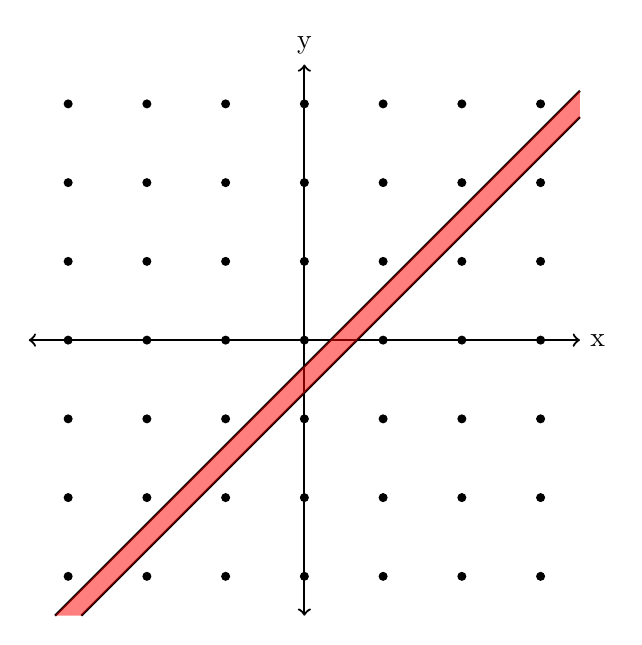
\begin{tikzpicture}
    %\draw[style=help lines,very thin] (-4, -4) grid (4, 4);
    \foreach \x in {-3, -2, ..., 3} {
      \foreach \y in {-3, -2, ..., 3} {
        \node[draw, circle, fill=black, inner sep=1pt] at (\x, \y) {};
      }
    }

    \draw[thick, ->] (0, 0) -- (3.5, 0) node[anchor=west] {x};
    \draw[thick, ->] (0, 0) -- (0, 3.5) node[anchor=south] {y};
    \draw[thick, ->] (0, 0) -- (-3.5, 0);
    \draw[thick, ->] (0, 0) -- (0, -3.5);


    \coordinate (C1LEFT) at (-3.167, -3.5);
    \coordinate (C1RIGHT) at (3.5, 3.167);
    \coordinate (C2LEFT) at (-2.833, -3.5);
    \coordinate (C2RIGHT) at (3.5, 2.833);
    \draw[thick] (C1LEFT) -- (C1RIGHT);
    \draw[thick] (C2LEFT) -- (C2RIGHT);
    \fill[fill=red, opacity=0.5]
      (C1LEFT) -- (C1RIGHT) -- (C2RIGHT) -- (C2LEFT) -- cycle;
  \end{tikzpicture}

  \label{bbloop}
  \caption{Graphical representation of the solutions of the problem
           \ref{pbloop}. The solutions of the relaxation lie in the red area.}
\end{figure}

In this case, the problem is unbounded and makes the branch-and-bound algorithm
loop. This is why we will try to add constraints of the form $-B \leqslant x_i
\leqslant B$ for all variable $x_i$ to bound the problem, at the condition that
the bounded problem admits a solution if and only if the original problem admits
a solution.

\subsection{Obtening bounds for ILPs and MILPs}
First of all, let us remark that if a linear problem contains only large
inequalities, it could be put in the form:

\begin{displaymath}
  \left\{
  \begin{array}{cccccl}
    a_{11} x_1 & + & ...    & + & a_{1n} x_n & \leqslant b_1 \\
               &   & \vdots &   &            &               \\
    a_{p1} x_0 & + & ...    & + & a_{pn} x_n & \leqslant b_p \\
  \end{array}
  \right.
\end{displaymath}

or in the matrix form $Ax \leqslant b$ with
$$A = (a_{ij})_{\substack{1 \leqslant i \leqslant n \\
                          1 \leqslant j \leqslant p}}$$ and
$b = (b_j)_{1 \leqslant j \leqslant p}$. We identify a valuation of $n$
variables to a vector of dimension $n$.

To derive bounds, we will use definitions and results that can be found in the
book of Schrijver \cite{Schrijver1998}.

\begin{definition}[Finitely Generated Cone]
  A set of points $C$ is a \textup{finitely generated cone}
  iff $C = \cone~\{x_0, ..., x_{n-1}\}$ where
  $$\cone~\{x_0, ..., x_{n-1}\} =
      \{\sum_{i<n} \lambda_i x_i~|~\lambda_0, ..., \lambda_{n-1} \leqslant 0\}
  $$
  for some $x_0, ..., x_{n-1}$.
\end{definition}

\begin{definition}[Polyhedral Cone]
  A set of points $C$ is a \textup{polyhedral cone}
  iff $C = \{x~|~Ax \leqslant 0\}$ for some matrix $A$.
\end{definition}

\begin{theorem}[Farkas-Minkowsky-Weyl Theorem]
  A set $C$ is a finitely generated cone iff is is a polyhedral cone.
\end{theorem}

\begin{definition}[Polyhedron]
  A set of points $P$ is a \textup{convex polyhedron} iff
  $$P = \{x~|~Ax \leqslant b\}$$
  for some matrix A and vector b.
\end{definition}

\begin{definition}[Polytope]
  A set of points $P$ is a \textup{polytope} iff it is the convex hull of a
  finite set $C = \{x_0, ..., x_{m-1}\}$, \textit{i.e}
  $$C = \{\sum_{i<m} \lambda_i x_i~|~\lambda_0, ..., \lambda_{m-1} \geqslant 0
                                     \wedge \sum_{i<m} \lambda_i = 1\}$$
\end{definition}

\begin{corollary}[Decomposition Theorem for Polyhedra]
  A set of points $P$ is a polyhedron iff there exists a polytope $C$ and a
  finitely generated cone $C$ such that $P = Q + C$.
\end{corollary}

To illustrate this theorem, let us take the following problem:
\begin{equation} \label{eqdecomp}
  \left\{
  \begin{array}{ccccc}
    -6x & + & 2y & \leqslant & 1  \\
    3x  & + & 2y & \geqslant & 11 \\
        &   & 2y & \geqslant & 1  \\
    2x  & - & 4y & \leqslant & 5
  \end{array}
  \right.
\end{equation}

As we have seen, the set of the solutions of this problem is a polyhedron. On
the figure \ref{figdecomp}, the polyhedron is represented by the red and blue
areas. As we can see, it is the sum of a polytope (the red triangle) and a cone
($\cone~\{u, v\}$).

\begin{figure}[h]
  \label{figdecomp}
  \centering

  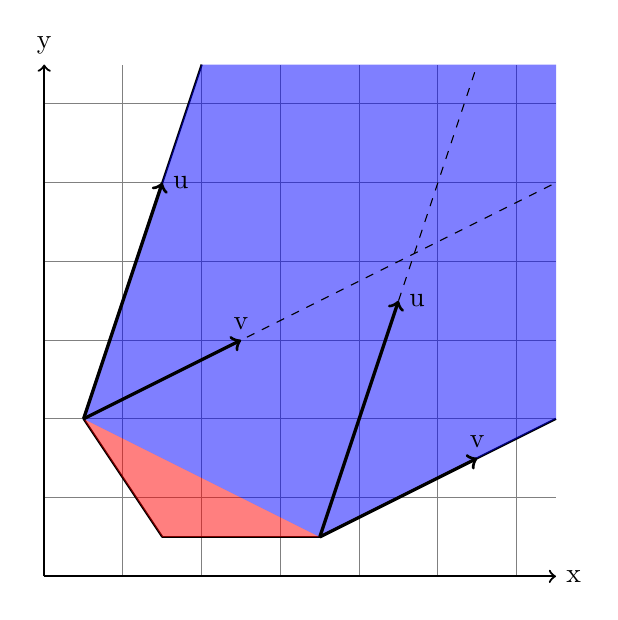
\begin{tikzpicture}
    \coordinate (extr) at (6.5, 6.5);
    \draw[style=help lines, thin] (0, 0) grid (extr);
    \draw[thick, ->] (0, 0) -- (6.5, 0) node[anchor=west] {x};
    \draw[thick, ->] (0, 0) -- (0, 6.5) node[anchor=south] {y};

    \coordinate (A) at (2, 6.5);
    \coordinate (B) at (0.5, 2);
    \coordinate (C) at (1.5, 0.5);
    \coordinate (D) at (3.5, 0.5);
    \coordinate (E) at (6.5, 2);
    \coordinate (B') at (6.5, 5);
    \coordinate (D') at (5.5, 6.5);
    \draw[thick] (A) -- (B);
    \draw[thick] (B) -- (C);
    \draw[thick] (C) -- (D);
    \draw[thick] (D) -- (E);
    \fill[fill=red, opacity=0.5] (B) -- (C) -- (D) -- cycle;
    \fill[fill=blue, opacity=0.5] (A) -- (B) -- (D) -- (E) -- (extr) --
                                  cycle;

    \draw[very thick, ->] (B) -- (1.5, 5) node[anchor=west] {u};
    \draw[very thick, ->] (B) -- (2.5, 3) node[anchor=south] {v};
    \draw[very thick, ->] (D) -- (4.5, 3.5) node[anchor=west] {u};
    \draw[very thick, ->] (D) -- (5.5, 1.5) node[anchor=south] {v};
    \draw[dashed] (B) -- (B');
    \draw[dashed] (D) -- (D');
  \end{tikzpicture}

  \caption{Decomposition of the polyhedron defined by the problem
           \ref{eqdecomp}}
\end{figure}

\begin{corollary}
  $P$ is a polytope iff $P$ is a bounded polyhedron.
\end{corollary}

\begin{definition}[Integer Hull]
  Given a polyhedron $P$, the \textup{integer hull} $P_I$ is the convex hull of
  the integral vectors of $P$, i.e $P_I = Hull (P \cap \mathbb{Z}^n\}$.
\end{definition}

\begin{theorem}
  For any rational polyhedron $P$, $P_I$ is a polyhedron. Moreover, if
  $P = Q + C$ with $Q$ a polytope and $C$ a cone, the there exists a polytope
  $Q'$ such that $P_I = Q' + C$.
\end{theorem}
\begin{proof}
  Let us decompose $P$ into $P = Q + C$ where
  $C = \cone~\{y_0, ..., y_{s-1}\}$. All the $y_i$ are rational vectors.
  Note that if we multiply them by positive constants, the cone is unchanged.
  This why, without loss of generality, we can assume that the $y_i$ are
  integral.

  Let us define
  $$B = \{\sum_{i < s} \mu_i y_i~|~0 \leqslant \mu_i \leqslant 1\}$$
  and show that $$P = (Q + B)_I + C$$

  The easy inclusion is the following:
  $$(Q + B)_I + C \subseteq P_I + C = P_I + C_I \subseteq (P + C)_I = P_I$$

  To prove the other inclusion, let us introduce $x \in P$.
  There exists $q \in Q$ and $\lambda_0, ..., \lambda_{s-1}
  \leqslant 0$ such that: $$x = q + \sum_{i < s} \lambda_i y_i$$ But for every
  $i$, $\lfloor \lambda_i \rfloor y_i$ is an integral vector, so
  $$x - \sum_{i<n} \lfloor \lambda_i \rfloor y_i=
      q + \sum_{i<n} (\lambda_i - \lfloor \lambda_i \rfloor) y_i$$
  is integral, and as $\sum_{i<n} (\lambda_i - \lfloor \lambda_i \rfloor) y_i$
  is contained in $B$:
  $$x - \sum_{i<n} \lfloor \lambda_i \rfloor y_i \in (Q + B)_I$$
  Finally: $x \in (Q + B)_I + C$

  $(Q + B)$ is bounded, so $(Q + B)_I$ is the convex hull of a finite set, it is
  a polytope. If we take $Q' = (Q + B)_I$, we have the result.
\end{proof}

A graphical representation of this proof is given in figure
\ref{integer_hull_decomp}. With again the polytope defined by the problem
\ref{eqdecomp}, the set boundary of the set $(Q + B)$ is represented
in red, $(Q + B)_I$ is represented in green. As we can see, $(Q + B)_I + C$ (the
red and yellow areas) is exactly the integer hull of the polyhedron.

\begin{figure}[h]
  \label{integer_hull_decomp}
  \centering

  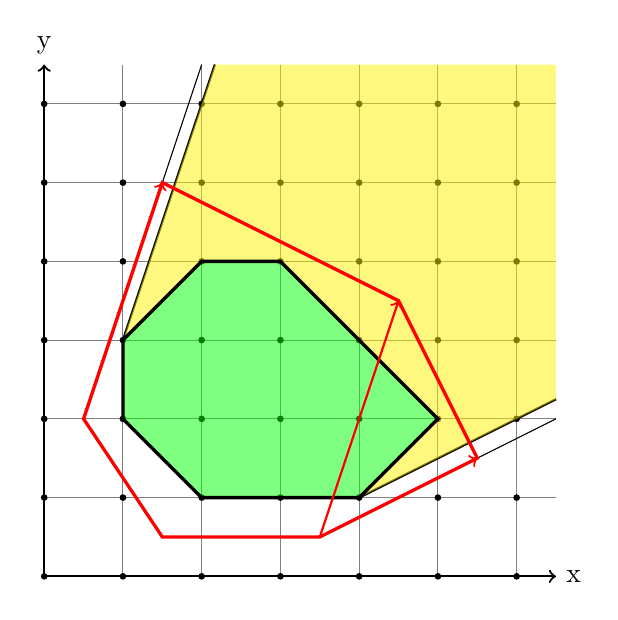
\begin{tikzpicture}
    \coordinate (extr) at (6.5, 6.5);
    \draw[style=help lines, thin] (0, 0) grid (extr);
    \draw[thick, ->] (0, 0) -- (6.5, 0) node[anchor=west] {x};
    \draw[thick, ->] (0, 0) -- (0, 6.5) node[anchor=south] {y};
    \foreach \x in {0, 1, ..., 6} {
      \foreach \y in {0, 1, ..., 6} {
        \node[draw, circle, fill=black, inner sep=0.7pt] at (\x, \y) {};
      }
    }

    \coordinate (A) at (2, 6.5);
    \coordinate (A') at (2.167, 6.5);
    \coordinate (B) at (0.5, 2);
    \coordinate (C) at (1.5, 0.5);
    \coordinate (D) at (3.5, 0.5);
    \coordinate (E) at (6.5, 2);
    \coordinate (E') at (6.5, 2.25);
    %\coordinate (B') at (6.5, 5);
    %\coordinate (D') at (5.167, 5.5);

    \coordinate (I) at (2, 4);
    \coordinate (J) at (1, 3);
    \coordinate (K) at (1, 2);
    \coordinate (L) at (2, 1);
    \coordinate (M) at (4, 1);
    \coordinate (N) at (5, 2);
    \coordinate (O) at (3, 4);

    \draw[thin] (A) -- (B);
    \draw[thin] (B) -- (C);
    \draw[thin] (C) -- (D);
    \draw[thin] (D) -- (E);

    \draw[thick] (A') -- (J);
    \draw[thick] (M) -- (E');

    \fill[fill=yellow, opacity=0.5]
      (A') -- (J) -- (I) -- (O) -- (N) -- (M) -- (E') -- (extr) -- cycle;
    \draw[red, very thick]
      (B) -- (C) -- (D) -- (5.5, 1.5) -- (4.5, 3.5) -- (1.5, 5) -- cycle;
    \draw[very thick, fill=green, fill opacity=0.5]
      (I) -- (J) -- (K) -- (L) -- (M) -- (N) -- (O) -- cycle;

    \draw[red, thick, ->] (B) -- (1.5, 5);
    \draw[red, thick, ->] (D) -- (4.5, 3.5);
    \draw[red, thick, ->] (D) -- (5.5, 1.5);
  \end{tikzpicture}

  \caption{Decomposition of the integer hull of the polytope defined by the
           problem \ref{eqdecomp}}
\end{figure}

With this result, we know that the problem has an integral solution iff it has
an integral solution in $Q'$ which is bounded. We now want to find a general
bound $B$ depending on the parameters of the problem.
In addition to the previous theorem, we need
integrality an bound hypotheses to $C$. Let us use the notations
$\llbracket a, b \rrbracket$ for the integers in the interval $[a, b]$.
We finally have the desired theorem:

\begin{theorem}
  If $P = \{x~|~Ax \leqslant b\}$ with
  $A \in \llbracket -m, m \rrbracket^{p \times n}$,
  $b \in \llbracket -m, m \rrbracket^p$ and $m \geqslant 1$, then
  $$P \cap \mathbb{Z}^n \neq \emptyset \Longleftrightarrow
  P \cap \llbracket -B, B \rrbracket^n \neq \emptyset$$ where
  $$B = (n + 1)! \cdot m^n$$
\end{theorem}

With the same ouline of proof, we can obtain a more general result that
encompasses MILPs and strict inequalities. If $I$ is a subset of
$\llbracket 1, n \rrbracket$:
\begin{theorem}
  If $P = \{x~|~Ax \leqslant b \cap A'x < b'\}$ with
  $A \in \llbracket -m, m \rrbracket^{p \times n}$,
  $b \in \llbracket -m, m \rrbracket^p$,
  $A' \in \llbracket -m, m \rrbracket^{p \times n}$,
  $b' \in \llbracket -m, m \rrbracket^p$ and $m \geqslant 1$, then

  $$\{x \in P~|~\forall i \in I.~x_i \in \mathbb{Z}\} \neq \emptyset
      \Longleftrightarrow
    \{x \in P~|~\forall i \in I.~x_i \in \llbracket -B, B \rrbracket\}
      \neq \emptyset$$
  where
  $$B = (n + 1)! \cdot m^n$$
\end{theorem}


\bibliographystyle{plain}
\bibliography{sources}

\appendix

\section{Example: an Execution of DPLL($T$)}
\label{dpll}
Suppose that we want to solve the formula $\Phi$ given in section \ref{smt}
using DPLL($T$). First, let us interpret $\Phi$ as a SAT-formula and find an
valuation that satisfies it. For example:
\begin{itemize}
  \item Arbitrarily affects $A$ to 1. Asserts the atom $A$. Get a checkpoints
    $c_1$.
  \item To solve the clause $(\neg A \vee B)$, we must affect $B$ to 1.
    Asserts the atom $B$. Get a checkpoint $c_2$.
  \item Affects $C$ to 1. Asserts the atom $C$. Get a checkpoint $c_3$.
  \item To solve the clause $(\neg C \vee D)$, we must affect $D$ to 1.
    Asserts the atom $D$. Get a checkpoint $c_4$.
\end{itemize}

Now, we have found an valuation that satisfies $\Phi$ interpreted as a
SAT-formula. But we need to check if this valuation is compatible with an
assignment in the theory of linear arithmetic. It means that we need to find an
assignment to the conjuction $A \wedge B \wedge C \wedge D$, which is equivalent
to the system:
\begin{displaymath}
  \left\{
  \begin{array}{ccccr}
    x  & + & y & \geqslant 3 & (A) \\
    x  &   &   & \leqslant 1 & (B) \\
       &   & y & \leqslant 1 & (C) \\
    y  & - & x & < 2         & (D) \\
  \end{array}
  \right.
\end{displaymath}

But this system has no solution. The procedure $\icheck$ may retun that the
constraints $A$, $B$ and $C$ are mutually incompatible. As these three
constraints cannot be satisfied simultaneously, an assignement that satisfies
$\Phi$ must violate at least one of these constraints, so we can deduce that the
clause $(\neg A \vee \neg B \vee \neg C)$ is true. Instead of solving $\Phi$, we
will try to solve $\Phi' = \Phi \wedge (\neg A \vee \neg B \vee \neg C)$. We
need to backtrack, but we can notice that we could bactrack just before
the choice to affect $C$ to 1 was made. So let us backtrack to $c_2$, where only
$A$ and $B$ are affected.

\begin{itemize}
  \item To solve the clause $(\neg A \vee \neg B \vee \neg C)$, we must affect
    $C$ to 0. Asserts the atom $\neg C$. Get a checkpoint $c'_3$.
  \item To solve the clause $(\neg A \vee C \vee D)$, we must affect $D$ to 1.
    Asserts the atom $D$. Get a checkpoint $c'_4$.
\end{itemize}

Again, we have a valuation that satisfies $\Phi'$ interpreted as a
SAT-formula. We have to find an assignement that satisfies the conjuction
$A \wedge B \wedge \neg C \wedge D$, which is equivalent
to the system:
\begin{displaymath}
  \left\{
  \begin{array}{ccccr}
    x  & + & y & \geqslant 3 & (A) \\
    x  &   &   & \leqslant 1 & (B) \\
       &   & y & > 1         & (\neg C) \\
    y  & - & x & < 2         & (D) \\
  \end{array}
  \right.
\end{displaymath}

$\icheck$ may return the assignement $(x=1, y=2)$. Finally, the formula $\Phi$
is satisfiable, and $(x=1, y=2) \vDash \Phi$.

\section{To move on another section} To do so, we will generalize the statements of
the previous theorems to incorporate bounds. 
\begin{theorem}[Generalized Farkas-Minkowsky-Weyl Theorem]
  A set $C$ is a finitely generated cone iff is is a polyhedral cone.

  Moreover, if $C = \cone~X$ with $X \subseteq \llbracket -m, m \rrbracket$
  and $m \geqslant 1$,
  then there exists a matrix $A \in \llbracket -B, B \rrbracket^{p \times n}$
  such that $$C = \{x~|~Ax \leqslant 0\}$$ with $$B = (n-1)! \cdot m^n$$
\end{theorem}

\begin{corollary}[Generalized Decomposition Theorem]
  A set of points $P$ is a polyhedron iff there exists a polytope $C$ and a
  finitely generated cone $C$ such that $P = Q + C$.

  Moreover, if $P = \{x~|~Ax \leqslant b\}$ with
  $A \in \llbracket -m, m \rrbracket^{p \times n}$ and
  $b \in \llbracket -m, m \rrbracket^p$, and $m \geqslant 1$,
  then there exists finite sets
  $Q \subseteq [-B, B]$ and $X \subseteq \llbracket -B, B \rrbracket$ such that
  $$P = hull~Q + \cone~X$$ with $$B = n! \cdot m^n$$
\end{corollary}



\end{document}
